\subsection{結果}
\subsubsection{客観評価1: ベースラインと提案手法の比較}
\label{sec4:sec:obj_1}
本節では,ベースラインと提案手法の比較を行う.比較手法は,以下の四つである.
\begin{enumerate}
    \item ベースライン
    \item ネットワークA
    \item ネットワークB(Randomized)
    \item ネットワークB(Pretrained)
\end{enumerate}
ベースラインは,提案手法におけるネットワークAで,メルスペクトログラムとHuBERT離散特徴量のみを予測するマルチタスク学習手法である.よって,損失関数は$\lossB$と同じである.ネットワークAは提案手法自体ではないが,その構成要素となっているため,ここでも客観評価指標を確認する.ネットワークB(Randomized)は,HuBERT Transformer層をランダム初期化した場合,ネットワークB(Pretrained)は,事前学習済み重みで初期化した場合である.これらを比較することで,HuBERT Transformer層の転移学習の有効性を調べた.

まず,損失関数の重み係数$\lossWeightHubDisc$を変化させた時の,客観評価指標の値を表\ref{sec4:tab:obj_weights}に示す.各手法の客観評価指標ごとに,最も優れた値を下線で示している.また,各手法ごとに最適だと判断した場合を太字で示している.

ベースラインでは,$\lossWeightHubDisc$が0.001のときにWERが最も低く,0.01のときに話者類似度が最も高くなった.現状WERの高さが特に課題であり,話者類似度はほとんど同じであったため,今回は0.001が最適だと判断した.図\ref{sec4:fig:learning_curve_baseline_val_losses}に学習曲線を示す.横軸がエポック数,縦軸が損失の値を表す.損失の値は各エポックにおける平均値である.実線は検証データに対する損失,点線は学習データに対する損失を表しており,線の色は$\lossWeightHubDisc$の違いを表す.また,丸いマーカーはテストデータの合成に用いたエポックにおける損失の値を表す.最適とした0.001の場合,学習データと検証データの両方において,メルスペクトログラムについてのMAE LossとHuBERT離散特徴量についてのCross Entropy Lossがバランスよく下がっていることがわかる。これに対し,客観評価指標が同程度であった0.0001と0.01の場合,学習曲線にも顕著な差は見られなかったから,妥当な結果だと考える.また,0.1と1.0では,0.01以下の場合と比較して話者類似度の低下が顕著であったが,この時学習データに対するメルスペクトログラムについてのMAE Lossが十分に下がり切らないまま,Early Stoppingによって学習が中断されていたことが分かる.これより,HuBERT離散特徴量が主に言語情報を反映している一方で、話者性を適切に反映するためにはメルスペクトログラムについてのMAE Lossが重要であることが示唆された.特に,学習データに対するフィッティングの程度が話者類似度に影響を与える可能性がある.最後に,$\lossWeightHubDisc$の値を大きくすることによって,HuBERT離散特徴量についてのCross Entropy Lossの下がり方が急峻になっていることがわかる.しかし,これと一貫性のある傾向は客観評価指標では見られなかった.

ネットワークAでは,提案手法の構成要素であるため最適な手法の選択は行わなかった.ベースラインとの違いはHuBERT中間特徴量についてのMAE Lossが損失に含まれることであるが,客観評価指標の値はベースラインと概ね同様であった.図\ref{sec4:fig:learning_curve_baseline_val_losses}に学習曲線を示す.これについてもベースラインと同様であり,客観評価指標の結果と合わせて妥当だと考える.

ネットワークB(Randomized)では,$\lossWeightHubDisc$が0.1の時にWERが最も低く,0.0001の時に話者類似度が最も高くなった.ここではWERの低さを優先し,0.1が最適だと判断した.図\ref{sec4:fig:learning_curve_method_2_val_losses}に学習曲線を示す.最適とした0.1の場合,学習データと検証データの両方において,メルスペクトログラムについてのMAE LossとHuBERT離散特徴量についてのCross Entropy Lossがバランスよく下がっていることがわかる。また,1.0では,0.1以下の場合と比較して話者類似度の低下が顕著であったが,この時学習データに対するメルスペクトログラムについてのMAE Lossが十分に下がり切らないまま,Early Stoppingによって学習が中断されていたことが分かる.これはベースラインと同様の傾向であった.最後に,$\lossWeightHubDisc$の値を大きくすることによって,HuBERT離散特徴量についてのCross Entropy Lossの下がり方が急峻になっていることがわかる.また,これに伴って0.0001から0.1まではWERが低下傾向にあり,これはベースラインと異なる傾向であった.

ネットワークB(Pretrained)では,$\lossWeightHubDisc$が0.1の時にWERが最も低くなった一方で,0.01以下の場合と比較したときの話者類似度の低下が顕著であり,ネットワークB(Randomized)とは異なる傾向であった.今回はWERが低いことを優先して,0.1が最適だと判断した.図\ref{sec4:fig:learning_curve_method_4_val_losses}に学習曲線を示す.ネットワークB(Randomized)と概ね同様であるが,$\lossWeightHubDisc = 0.1$の場合に学習データに対するメルスペクトログラムについてのMAE Lossが下がりきっていない点が異なる.その他のネットワークにおいて,この傾向は話者類似度の低下傾向に一致していることから,ネットワークB(Randomized)のようにWERを低下させつつ話者類似度を高い値で保つことができなかったのは,学習の結果として妥当だと考える.初期値の違いによってこの傾向の違いが現れているから,本実験条件下においてはHuBERTの事前学習済み重みが有効でなかったと考えられる.

最後に,最適なチューニングをした場合における手法ごとの比較を行った結果を表\ref{sec4:tab:obj_method_comp}に示す.分析合成は,原音声から計算した特徴量を入力としてボコーダで逆変換した合成音声であり,本実験下において合成音声により達成され得る上限を表す.ベースライン,ネットワークB(Randomized),ネットワークB(Pretrained)は,上記の議論で最適なチューニングだと判断したものを選択しており,これらの中で最も優れた値を下線で示した.これより,提案手法であるネットワークB(Randomized)は,ベースラインに対してWERを9.3\%低下させ,話者類似度を0.004向上させたことが分かる.一方,ネットワークB(Pretrained)はWERを10.4\%低下させたが,話者類似度は0.058低下したことが分かる.また,ネットワークB(Randomized)とネットワークB(Pretrained)を比較すると,ネットワークB(Pretrained)の方がWERは1.1\%低いが,話者類似度が0.062低いことが分かる.実際に音声を聞いてみると,音声に不自然なノイズが含まれており,原音声に対する類似性が下がっていることが確認された.よって,HuBERTの事前学習済み重みを初期値としたHuBERT Transformer層の転移学習は,本実験条件下においては有効でなかったと考えられる.以上より,本実験の客観評価指標による評価結果としては,$\lossWeightHubDisc = 0.1$としたネットワークB(Randomized)が最も優れていたと考える.

\begin{table}[bt]
    \centering
    \caption{損失関数の重み係数$\lossWeightHubDisc$による客観評価指標の変化}
    \label{sec4:tab:obj_weights}
    \begin{center}
        \renewcommand{\arraystretch}{1.0} % 行の高さ調整
        \setlength{\tabcolsep}{8pt}      % 列の幅調整
        \scalebox{1.0}{
            \begin{tabular}{|c|l|rr|}
                \hline
                \multicolumn{1}{|c|}{手法}     & \multicolumn{1}{c|}{$\lossWeightHubDisc$} & \multicolumn{1}{c}{WER [\%]} & \multicolumn{1}{c|}{話者類似度} \\
                \hline
                ベースライン                       & 0.0001                                    & 57.3                         & 0.833                      \\
                \textbf{ベースライン}              & \textbf{0.001}                            & \underline{\textbf{54.6}}    & \textbf{0.836}             \\
                ベースライン                       & 0.01                                      & 56.2                         & \underline{0.837}          \\
                ベースライン                       & 0.1                                       & 58.2                         & 0.784                      \\
                ベースライン                       & 1                                         & 59.0                         & 0.685                      \\
                \hline
                ネットワークA                      & 0.0001                                    & 55.4                         & 0.841                      \\
                ネットワークA                      & 0.001                                     & 55.1                         & 0.842                      \\
                ネットワークA                      & 0.01                                      & \underline{53.4}             & \underline{0.843}          \\
                ネットワークA                      & 0.1                                       & 54.6                         & 0.809                      \\
                ネットワークA                      & 1                                         & 58.7                         & 0.698                      \\
                \hline
                ネットワークB(Randomized)          & 0.0001                                    & 60.6                         & \underline{0.852}          \\
                ネットワークB(Randomized)          & 0.001                                     & 56.7                         & 0.829                      \\
                ネットワークB(Randomized)          & 0.01                                      & 54.4                         & 0.847                      \\
                \textbf{ネットワークB(Randomized)} & \textbf{0.1}                              & \underline{\textbf{45.3}}    & \textbf{0.840}             \\
                ネットワークB(Randomized)          & 1                                         & 45.5                         & 0.712                      \\
                \hline
                ネットワークB(Pretrained)          & 0.0001                                    & 60.1                         & 0.841                      \\
                ネットワークB(Pretrained)          & 0.001                                     & 57.1                         & 0.839                      \\
                ネットワークB(Pretrained)          & 0.01                                      & 56.8                         & \underline{0.860}          \\
                \textbf{ネットワークB(Pretrained)} & \textbf{0.1}                              & \underline{\textbf{44.2}}    & \textbf{0.778}             \\
                ネットワークB(Pretrained)          & 1                                         & 48.1                         & 0.685                      \\
                \hline
            \end{tabular}
        }
    \end{center}
\end{table}

\begin{figure}[bt]
    \centering
    \begin{subfigure}{\linewidth}
        \centering
        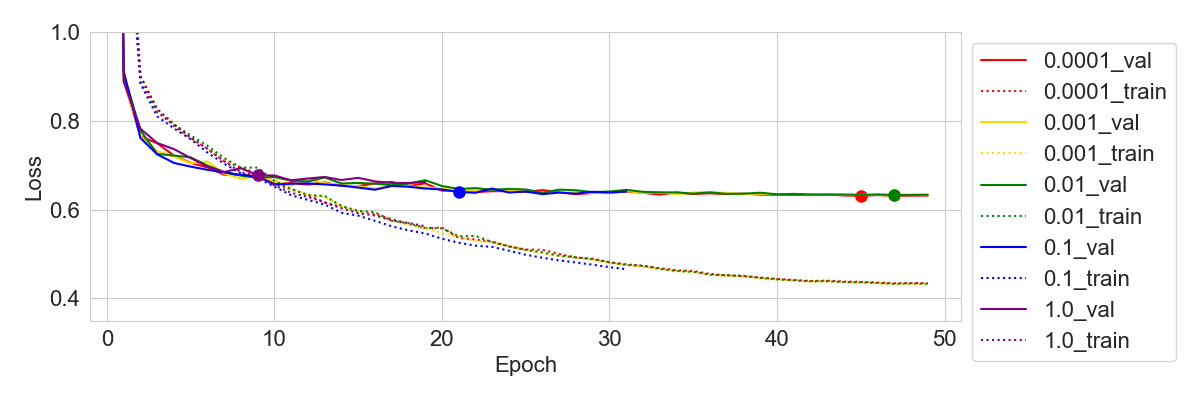
\includegraphics[height=55mm]{./figure/sec4/learning_curves/0/mel_loss.png}
        \caption{メルスペクトログラムについてのMAE Loss}
        \label{sec4:fig:learning_curve_baseline_val_mel_loss}
    \end{subfigure}
    \begin{subfigure}{\linewidth}
        \centering
        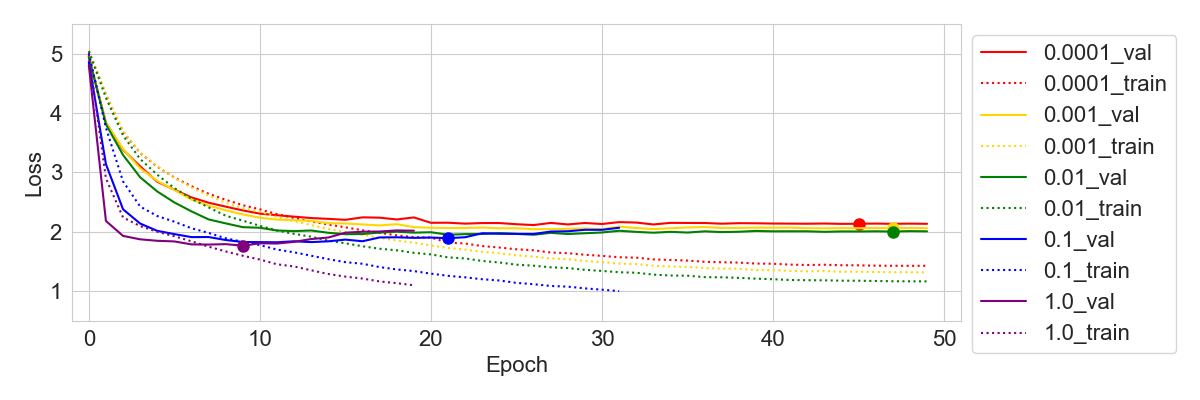
\includegraphics[height=55mm]{./figure/sec4/learning_curves/0/ssl_feature_cluster_loss.png}
        \caption{HuBERT離散特徴量についてのCross Entropy Loss}
        \label{sec4:fig:learning_curve_baseline_val_ssl_feature_cluster_loss}
    \end{subfigure}
    \begin{subfigure}{\linewidth}
        \centering
        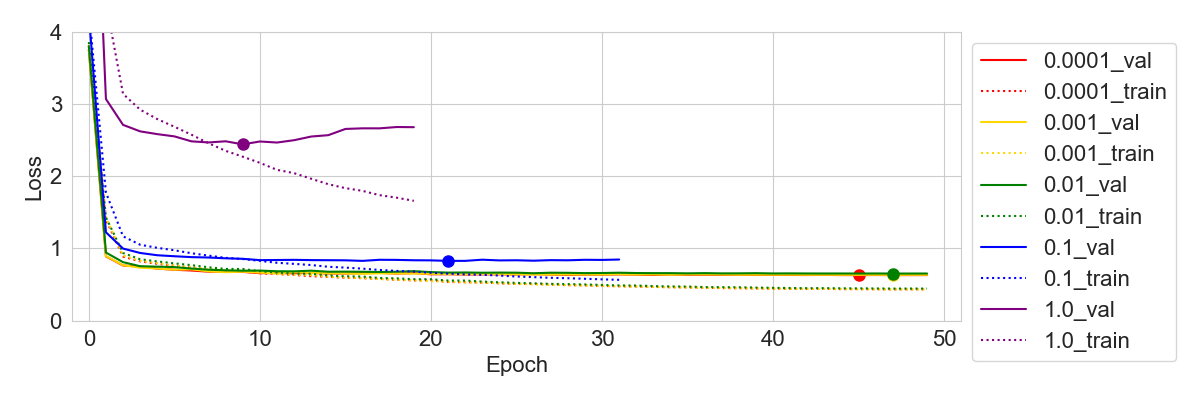
\includegraphics[height=55mm]{./figure/sec4/learning_curves/0/total_loss.png}
        \caption{損失の合計値}
        \label{sec4:fig:learning_curve_baseline_val_total_loss}
    \end{subfigure}
    \caption{ベースラインにおける学習曲線}
    \label{sec4:fig:learning_curve_baseline_val_losses}
\end{figure}

\begin{figure}[bt]
    \centering
    \begin{subfigure}{\linewidth}
        \centering
        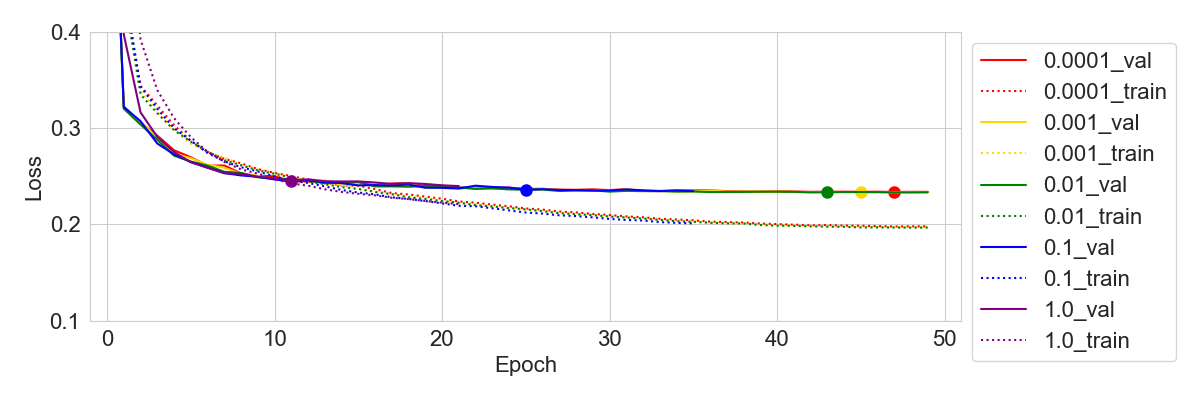
\includegraphics[height=45mm]{./figure/sec4/learning_curves/1/ssl_conv_feature_loss.png}
        \caption{HuBERT中間特徴量についてのMAE Loss}
        \label{sec4:fig:learning_curve_method_1_val_ssl_conv_feature_loss}
    \end{subfigure}
    \begin{subfigure}{\linewidth}
        \centering
        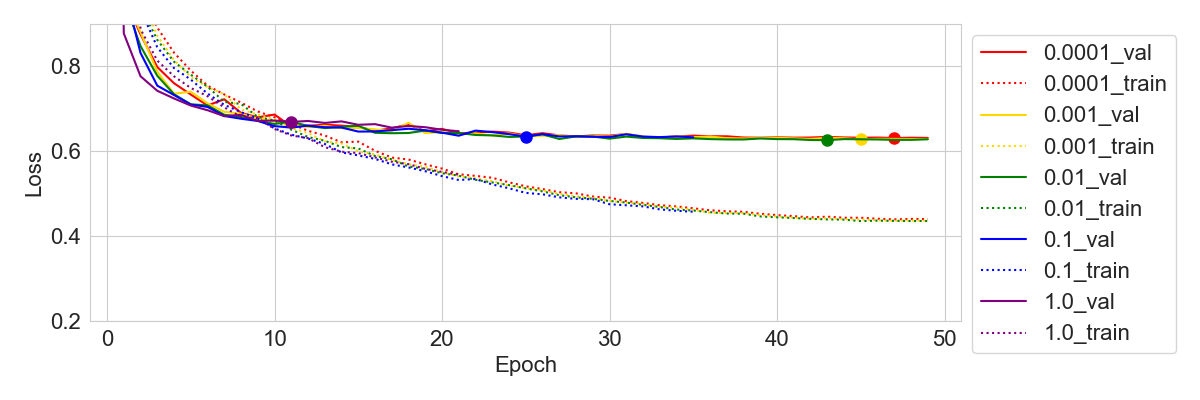
\includegraphics[height=45mm]{./figure/sec4/learning_curves/1/mel_loss.png}
        \caption{メルスペクトログラムについてのMAE Loss}
        \label{sec4:fig:learning_curve_method_1_val_mel_loss}
    \end{subfigure}
    \begin{subfigure}{\linewidth}
        \centering
        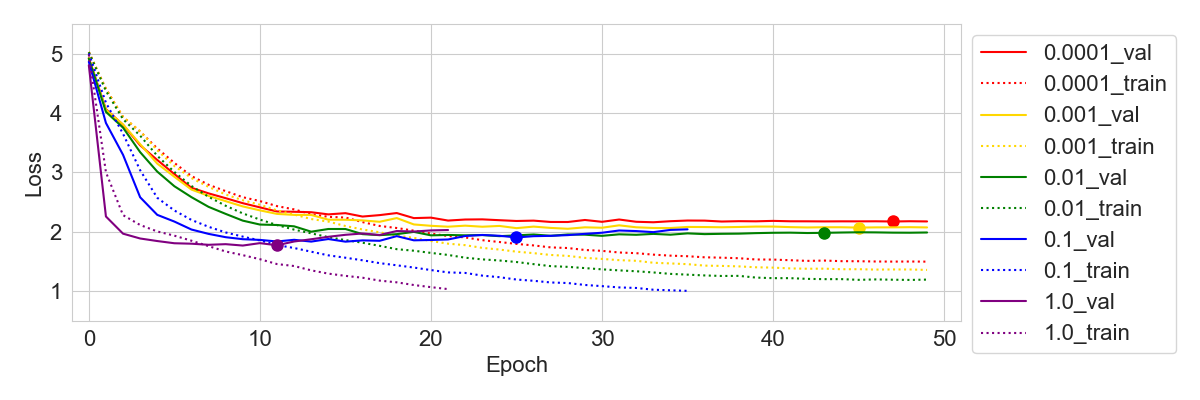
\includegraphics[height=45mm]{./figure/sec4/learning_curves/1/ssl_feature_cluster_loss.png}
        \caption{HuBERT離散特徴量についてのCross Entropy Loss}
        \label{sec4:fig:learning_curve_method_1_val_ssl_feature_cluster_loss}
    \end{subfigure}
    \begin{subfigure}{\linewidth}
        \centering
        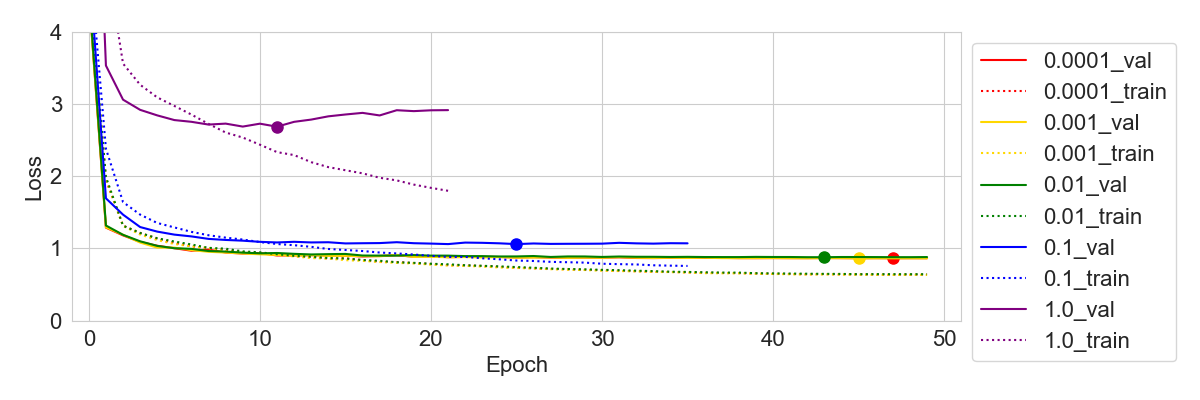
\includegraphics[height=45mm]{./figure/sec4/learning_curves/1/total_loss.png}
        \caption{損失の合計値}
        \label{sec4:fig:learning_curve_method_1_val_total_loss}
    \end{subfigure}
    \caption{ネットワークAにおける学習曲線}
    \label{sec4:fig:learning_curve_method_1_val_losses}
\end{figure}

\begin{figure}[bt]
    \centering
    \begin{subfigure}{\linewidth}
        \centering
        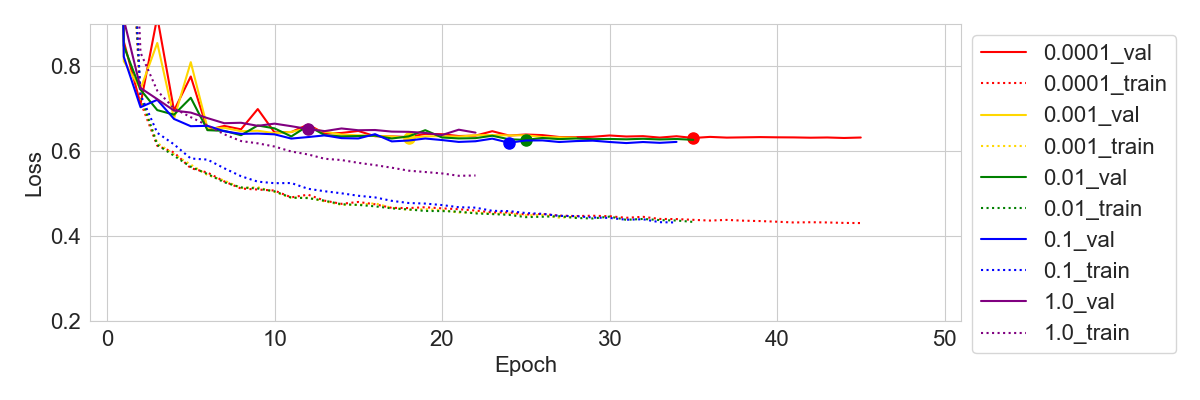
\includegraphics[height=55mm]{./figure/sec4/learning_curves/2/mel_loss.png}
        \caption{メルスペクトログラムについてのMAE Loss}
        \label{sec4:fig:learning_curve_method_2_val_mel_loss}
    \end{subfigure}
    \begin{subfigure}{\linewidth}
        \centering
        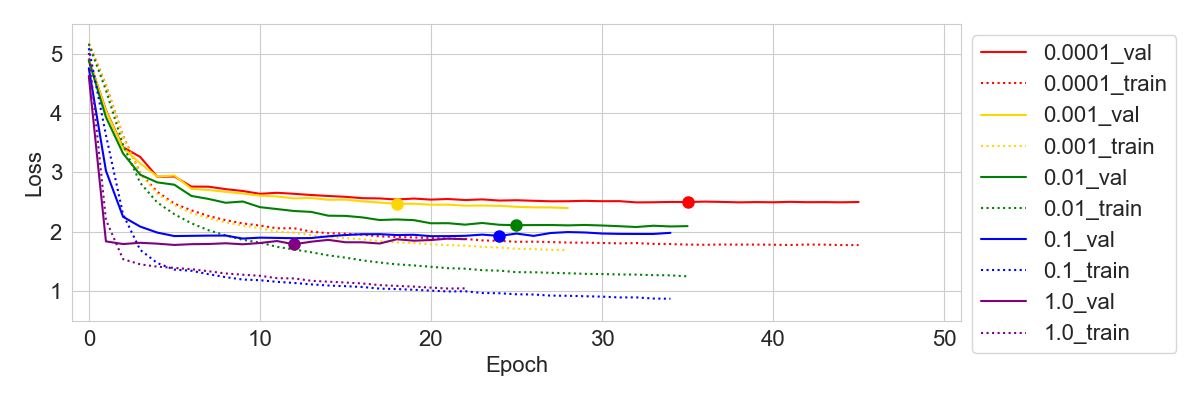
\includegraphics[height=55mm]{./figure/sec4/learning_curves/2/ssl_feature_cluster_loss.png}
        \caption{HuBERT離散特徴量についてのCross Entropy Loss}
        \label{sec4:fig:learning_curve_method_2_val_ssl_feature_cluster_loss}
    \end{subfigure}
    \begin{subfigure}{\linewidth}
        \centering
        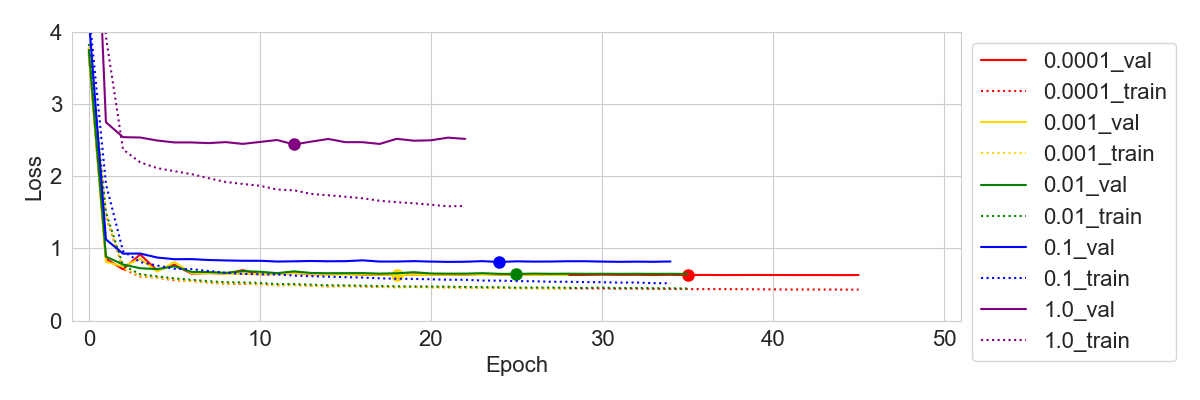
\includegraphics[height=55mm]{./figure/sec4/learning_curves/2/total_loss.png}
        \caption{損失の合計値}
        \label{sec4:fig:learning_curve_method_2_val_total_loss}
    \end{subfigure}
    \caption{ネットワークB(Randomized)における学習曲線}
    \label{sec4:fig:learning_curve_method_2_val_losses}
\end{figure}

\begin{figure}[bt]
    \centering
    \begin{subfigure}{\linewidth}
        \centering
        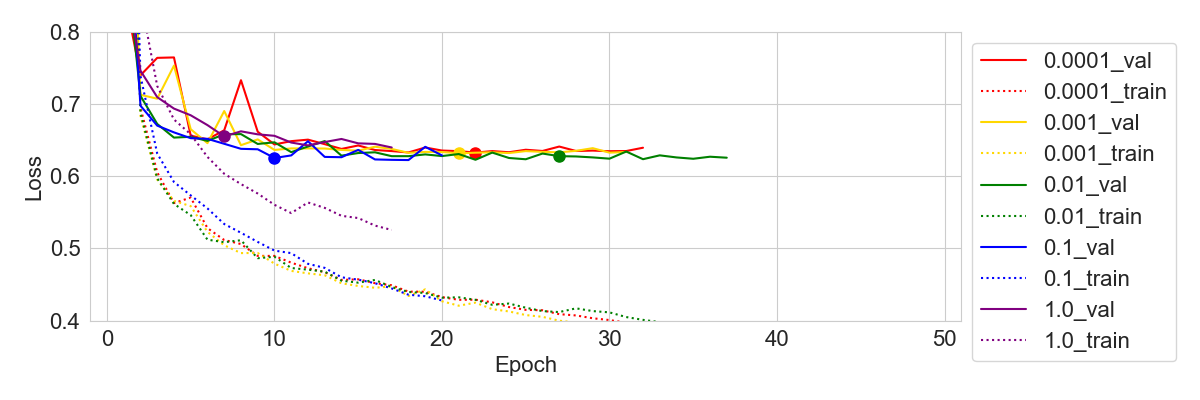
\includegraphics[height=55mm]{./figure/sec4/learning_curves/4/mel_loss.png}
        \caption{メルスペクトログラムについてのMAE Loss}
        \label{sec4:fig:learning_curve_method_4_val_mel_loss}
    \end{subfigure}
    \begin{subfigure}{\linewidth}
        \centering
        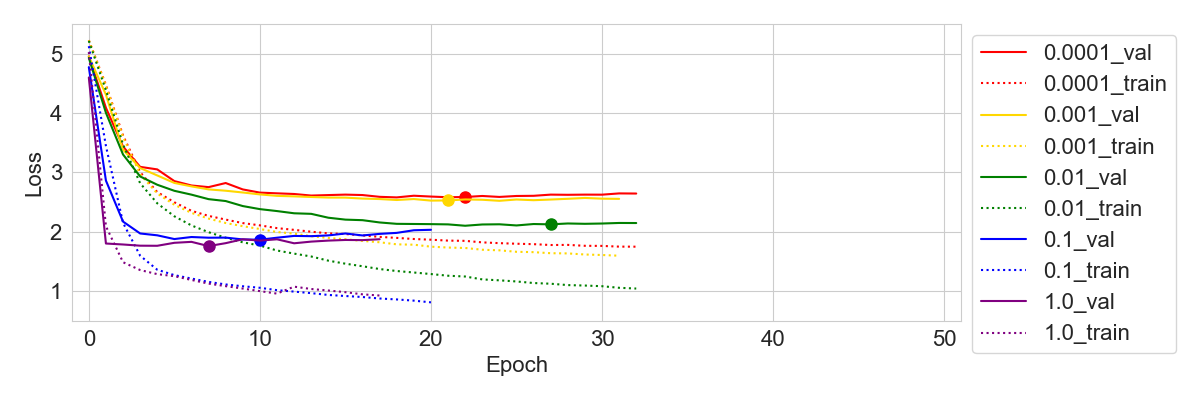
\includegraphics[height=55mm]{./figure/sec4/learning_curves/4/ssl_feature_cluster_loss.png}
        \caption{HuBERT離散特徴量についてのCross Entropy Loss}
        \label{sec4:fig:learning_curve_method_4_val_ssl_feature_cluster_loss}
    \end{subfigure}
    \begin{subfigure}{\linewidth}
        \centering
        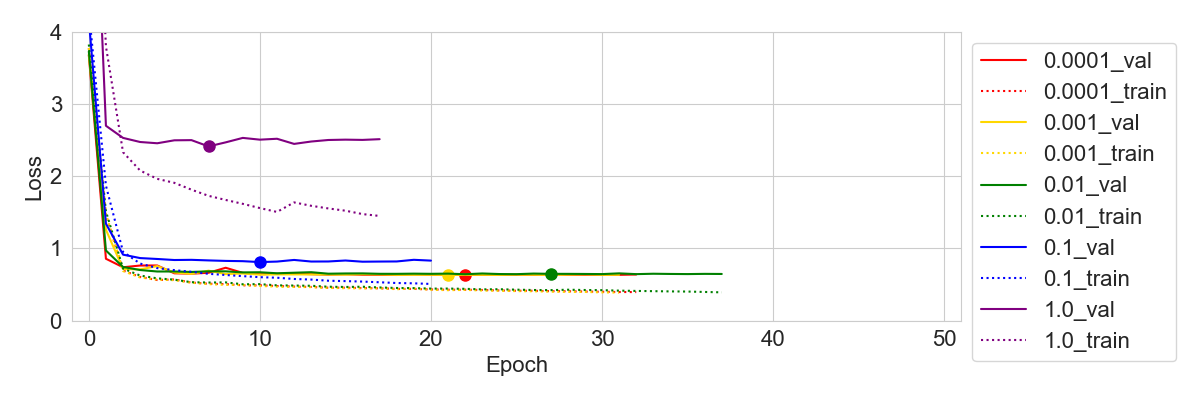
\includegraphics[height=55mm]{./figure/sec4/learning_curves/4/total_loss.png}
        \caption{損失の合計値}
        \label{sec4:fig:learning_curve_method_4_val_total_loss}
    \end{subfigure}
    \caption{ネットワークB(Pretrained)における学習曲線}
    \label{sec4:fig:learning_curve_method_4_val_losses}
\end{figure}

\begin{table}[bt]
    \centering
    \caption{最適なチューニングをした場合における手法ごとの比較}
    \label{sec4:tab:obj_method_comp}
    \begin{center}
        \renewcommand{\arraystretch}{1.0} % 行の高さ調整
        \setlength{\tabcolsep}{8pt}      % 列の幅調整
        \scalebox{1.0}{
            \begin{tabular}{|c|l|rr|}
                \hline
                \multicolumn{1}{|c|}{手法} & \multicolumn{1}{c|}{$\lossWeightHubDisc$} & \multicolumn{1}{c}{WER [\%]} & \multicolumn{1}{c|}{話者類似度} \\
                \hline
                ベースライン                   & 0.001                                     & 54.6                         & 0.836                      \\
                ネットワークB(Randomized)      & 0.1                                       & 45.3                         & 0.840                      \\
                ネットワークB(Pretrained)      & 0.1                                       & \underline{44.2}             & 0.778                      \\
                \hline
                分析合成                     & \multicolumn{1}{c|}{-}                    & 3.7                          & 0.956                      \\
                原音声                      & \multicolumn{1}{c|}{-}                    & 3.7                          & 1.000                      \\
                \hline
            \end{tabular}
        }
    \end{center}
\end{table}

\clearpage

\subsubsection{客観評価2: 提案手法のさらなる検討}
\label{sec4:sec:obj_2}
\ref{sec4:sec:obj_1}節において良好な結果を示したのはネットワークB(Randomized)であったが,これはHuBERTの転移学習による改善を狙った当初の仮説に反する結果であった.これに対し,本節では良好な結果を示したネットワークB(Randomized)に焦点を当てたさらなる検討の結果を述べる.

まず,HuBERT Transformer層への入力特徴量について検討した.\ref{sec4:sec:obj_1}節では事前学習済み重みを用いることの有効性を調べる目的があったため,入力特徴量はHuBERTの事前学習時に揃えて,HuBERT中間特徴量とした.しかし,ネットワークB(Randomized)は事前学習済み重みを利用しないため,HuBERT中間特徴量を入力とすることが意味をなしているか不明である.これに対し,ネットワークAからマルチタスク学習によって同時に予測される,メルスペクトログラムとHuBERT離散特徴量に対するロジットを入力とする場合を比較した.メルスペクトログラムは,時間方向に隣接した2フレームを次元方向に積むことで160次元50 Hzの特徴量に変換し,HuBERT離散特徴量に対するロジットは101次元50 Hzの特徴量としてそのまま用いた.これらを次元方向に結合することで261次元の特徴量を構成し,全結合層を通してHuBERT中間特徴量と同じ768次元に変換することで,HuBERT Transformer層への入力とした.結果を表\ref{sec4:tab:obj_weights_networkb_input_comparison}に示す.新たに検討した手法はネットワークB(Randomized・Mel-HuB)とし,$\lossWeightHubDisc = 0.001$の場合が最適だと判断した.これより,ネットワークB(Randomized・Mel-HuB)はネットワークB(Randomized)よりも話者類似度は0.005高いが,WERは10.1\%高いことが分かる.図\ref{sec4:fig:learning_curve_method_6_val_losses}にネットワークB(Randomized・Mel-HuB)の学習曲線を示す.最適とした0.001の場合,学習データと検証データの両方において,メルスペクトログラムについてのMAE LossとHuBERT離散特徴量についてのCross Entropy Lossがバランスよく下がっていることがわかる。また,ネットワークB(Randomized)では,$\lossWeightHubDisc$の値を大きくすることによって,HuBERT離散特徴量についてのCross Entropy Lossの下がり方が急峻になり,これに伴って0.0001から0.1まではWERが低下傾向にあった.これに対し,ネットワークB(Randomized・Mel-HuB)ではHuBERT離散特徴量についてのCross Entropy Lossの下がり方が急峻になる傾向は同様に見られるが,WERの低下傾向は見られなかった.以上より,HuBERT中間特徴量は,メルスペクトログラムとHuBERT離散特徴量のロジットから構成した特徴量と比較して,ネットワークBの推定精度改善につながるより良い入力特徴量であったと考えられる.

\begin{table}[bt]
    \centering
    \caption{HuBERT Transformer層への入力特徴量を変化させた場合の比較}
    \label{sec4:tab:obj_weights_networkb_input_comparison}
    \begin{center}
        \renewcommand{\arraystretch}{1.0} % 行の高さ調整
        \setlength{\tabcolsep}{8pt}      % 列の幅調整
        \scalebox{0.98}{
            \begin{tabular}{|c|l|rr|}
                \hline
                \multicolumn{1}{|c|}{手法}             & \multicolumn{1}{c|}{$\lossWeightHubDisc$} & \multicolumn{1}{c}{WER [\%]} & \multicolumn{1}{c|}{話者類似度} \\
                \hline
                ネットワークB(Randomized・Mel-HuB)          & 0.0001                                    & 59.5                         & 0.840                      \\
                \textbf{ネットワークB(Randomized・Mel-HuB)} & \textbf{0.001}                            & \textbf{55.4}                & \underline{\textbf{0.845}} \\
                ネットワークB(Randomized・Mel-HuB)          & 0.01                                      & 56.2                         & 0.803                      \\
                ネットワークB(Randomized・Mel-HuB)          & 0.1                                       & 57.7                         & 0.795                      \\
                ネットワークB(Randomized・Mel-HuB)          & 1                                         & 58.1                         & 0.711                      \\
                \hline
                ネットワークB(Randomized)                  & 0.1                                       & \underline{45.3}             & 0.840                      \\
                \hline
            \end{tabular}
        }
    \end{center}
\end{table}

\begin{figure}[bt]
    \centering
    \begin{subfigure}{\linewidth}
        \centering
        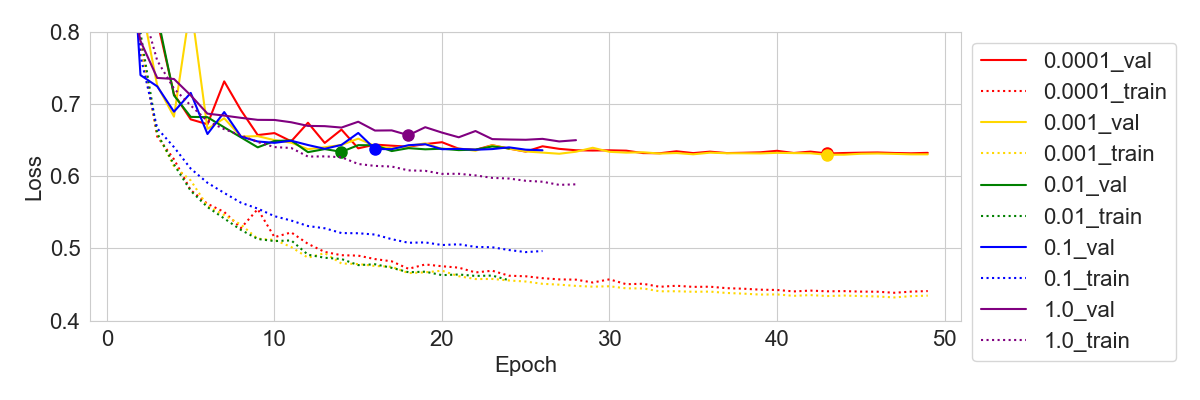
\includegraphics[height=55mm]{./figure/sec4/learning_curves/6/mel_loss.png}
        \caption{メルスペクトログラムについてのMAE Loss}
        \label{sec4:fig:learning_curve_method_6_val_mel_loss}
    \end{subfigure}
    \begin{subfigure}{\linewidth}
        \centering
        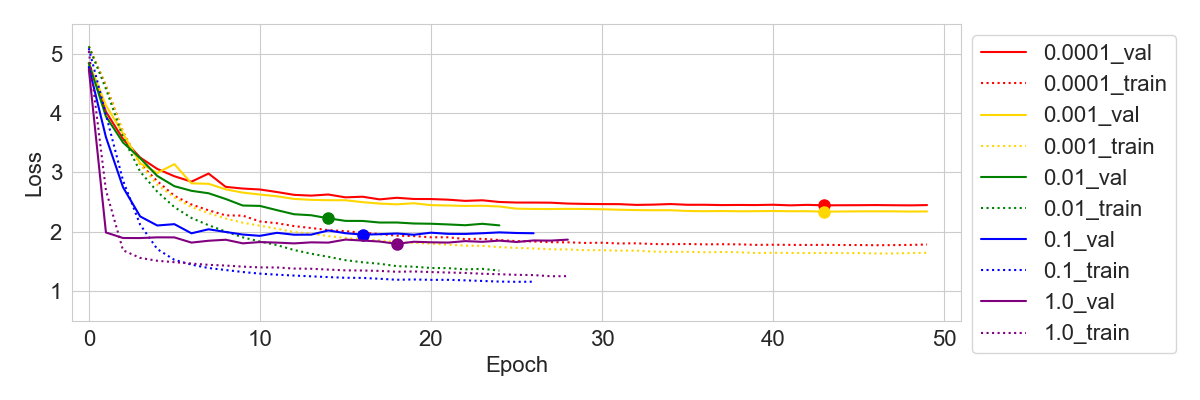
\includegraphics[height=55mm]{./figure/sec4/learning_curves/6/ssl_feature_cluster_loss.png}
        \caption{HuBERT離散特徴量についてのCross Entropy Loss}
        \label{sec4:fig:learning_curve_method_6_val_ssl_feature_cluster_loss}
    \end{subfigure}
    \begin{subfigure}{\linewidth}
        \centering
        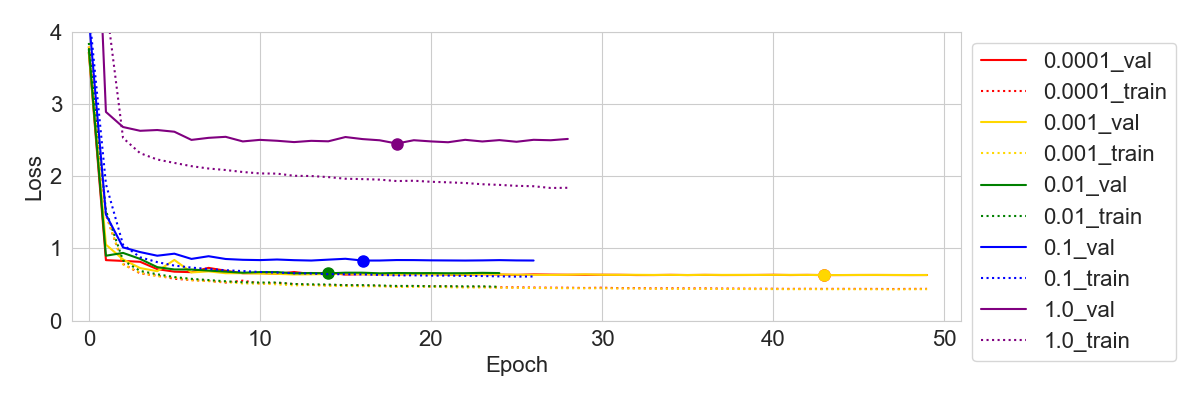
\includegraphics[height=55mm]{./figure/sec4/learning_curves/6/total_loss.png}
        \caption{損失の合計値}
        \label{sec4:fig:learning_curve_method_6_val_total_loss}
    \end{subfigure}
    \caption{ネットワークB(Randomized・Mel-HuB)における学習曲線}
    \label{sec4:fig:learning_curve_method_6_val_losses}
\end{figure}

次に,HuBERT中間特徴量をネットワークBに与えている,ネットワークAの学習方法を検討した.ここでは,これまでネットワークAで採用していたHuBERT中間特徴量,メルスペクトログラム,HuBERT離散特徴量を予測するマルチタスク学習に対し,HuBERT中間特徴量のみを予測するシングルタスク学習の場合を比較した.結果を表\ref{sec4:tab:obj_weights_networka_multitask}に示す.新たに検討した手法はネットワークB(Randomized・A-SingleTask)とし,$\lossWeightHubDisc = 0.1$の場合が最適だと判断した.これより,ネットワークB(Randomized・A-SingleTask)はネットワークB(Randomized)よりもWERが2.8\%低く,話者類似度は0.007高いことがわかる.図\ref{sec4:fig:learning_curve_method_9_val_losses}にネットワークB(Randomized・A-SingleTask)の学習曲線を示す.ネットワークB(Randomized)と同様の傾向であるから,客観評価指標の値が大きく変わらなかったことは妥当だと考える.以上より,ネットワークAではネットワークBの入力に必要なHuBERT中間特徴量のみを推定する方が,ネットワークB(Randomized)に対してより良い入力特徴量を与えられるのだと考えられる.

\begin{table}[bt]
    \centering
    \caption{ネットワークAにおけるマルチタスク学習の有無による比較}
    \label{sec4:tab:obj_weights_networka_multitask}
    \begin{center}
        \renewcommand{\arraystretch}{1.0} % 行の高さ調整
        \setlength{\tabcolsep}{8pt}      % 列の幅調整
        \scalebox{0.99}{
            \begin{tabular}{|c|l|rr|}
                \hline
                \multicolumn{1}{|c|}{手法}                  & \multicolumn{1}{c|}{$\lossWeightHubDisc$} & \multicolumn{1}{c}{WER [\%]} & \multicolumn{1}{c|}{話者類似度} \\
                \hline
                ネットワークB(Randomized・A-SingleTask)          & 0.0001                                    & 54.0                         & \underline{0.867}          \\
                ネットワークB(Randomized・A-SingleTask)          & 0.001                                     & 52.2                         & 0.865                      \\
                ネットワークB(Randomized・A-SingleTask)          & 0.01                                      & 51.8                         & 0.843                      \\
                \textbf{ネットワークB(Randomized・A-SingleTask)} & \textbf{0.1}                              & \underline{\textbf{42.5}}    & \textbf{0.847}             \\
                ネットワークB(Randomized・A-SingleTask)          & 1                                         & 43.0                         & 0.768                      \\
                \hline
                ネットワークB(Randomized)                       & 0.1                                       & 45.3                         & 0.840                      \\
                \hline
            \end{tabular}
        }
    \end{center}
\end{table}

\begin{figure}[bt]
    \centering
    \begin{subfigure}{\linewidth}
        \centering
        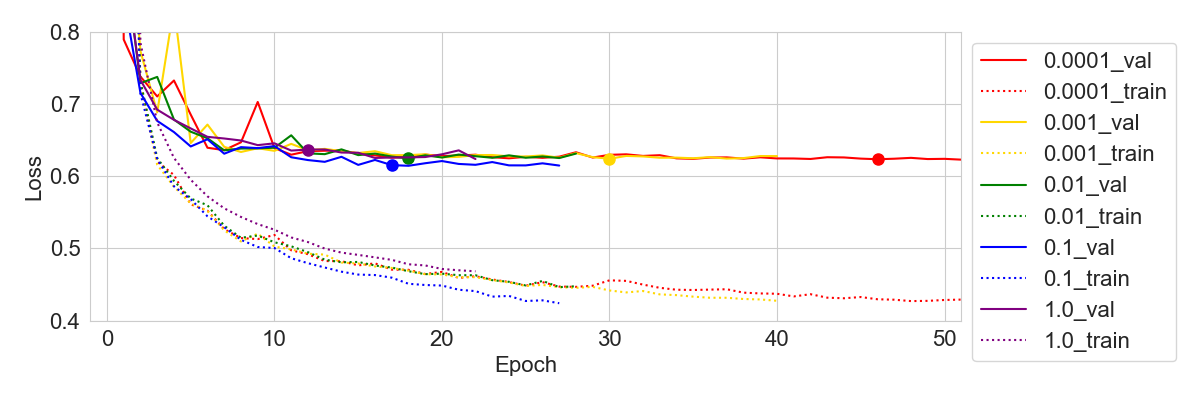
\includegraphics[height=55mm]{./figure/sec4/learning_curves/9/mel_loss.png}
        \caption{メルスペクトログラムについてのMAE Loss}
        \label{sec4:fig:learning_curve_method_9_val_mel_loss}
    \end{subfigure}
    \begin{subfigure}{\linewidth}
        \centering
        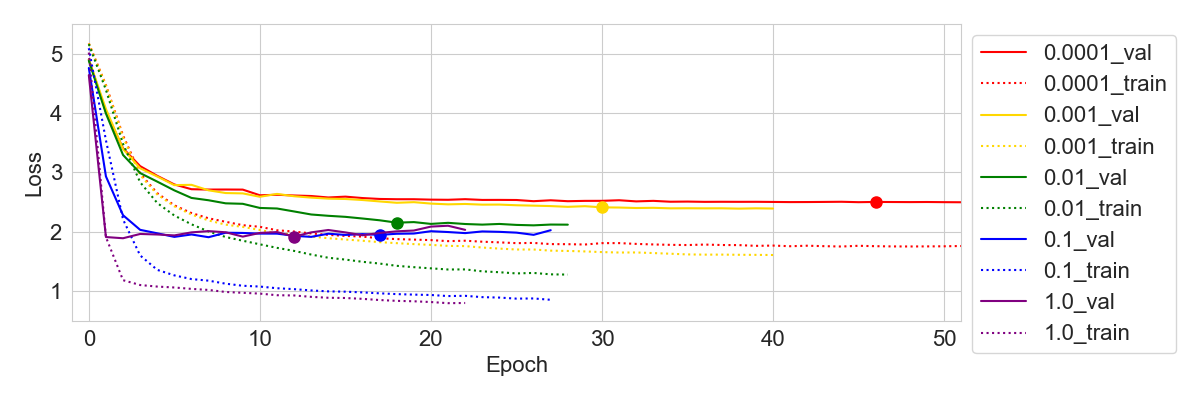
\includegraphics[height=55mm]{./figure/sec4/learning_curves/9/ssl_feature_cluster_loss.png}
        \caption{HuBERT離散特徴量についてのCross Entropy Loss}
        \label{sec4:fig:learning_curve_method_9_val_ssl_feature_cluster_loss}
    \end{subfigure}
    \begin{subfigure}{\linewidth}
        \centering
        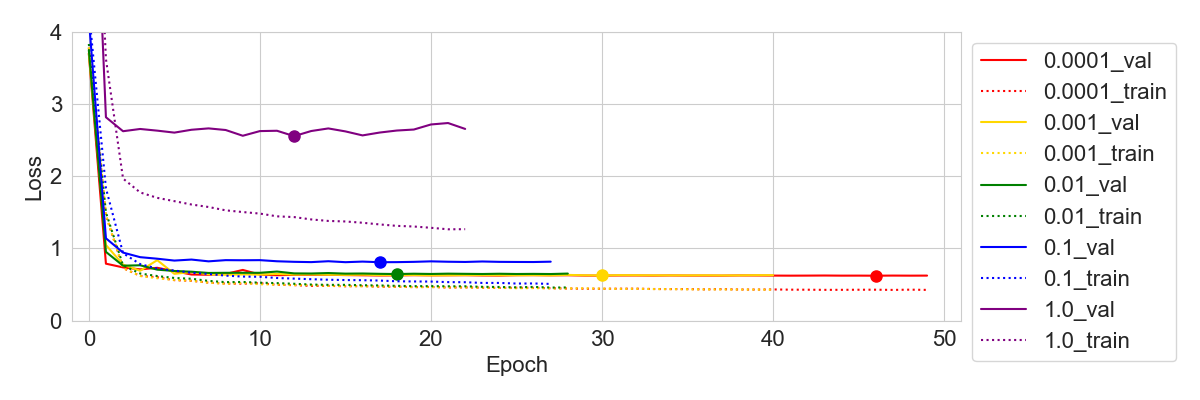
\includegraphics[height=55mm]{./figure/sec4/learning_curves/9/total_loss.png}
        \caption{損失の合計値}
        \label{sec4:fig:learning_curve_method_9_val_total_loss}
    \end{subfigure}
    \caption{ネットワークB(Randomized・A-SingleTask)における学習曲線}
    \label{sec4:fig:learning_curve_method_9_val_losses}
\end{figure}

最後に,これまでネットワークAとネットワークBを二段階で学習させたのに対し,ネットワークAからネットワークBまでを一度に学習させる方法を検討した.これにより,HuBERT中間特徴量に表現力を制限させないことで,さらなる精度改善を狙った.ここでは,ネットワークBの出力に対する損失関数$\lossB$のみを用いて学習させ,ネットワークAの出力は単にネットワークBへの入力とした.ネットワークAおよびネットワークB(Randomized)を未学習の状態で初期化した場合の結果を表\ref{sec4:tab:obj_weights_e2e_randomized}に示す.新たに検討した手法はネットワークE2E(Randomized)とし,$\lossWeightHubDisc = 0.1$が最適だと判断した.これより,ネットワークE2E(Randomized)はネットワークB(Randomized・A-SingleTask)よりもWERが20.0\%高く,話者類似度は0.080低いことがわかる.図\ref{sec4:fig:learning_curve_method_7_val_losses}に学習曲線を示す.二段階で学習させたネットワークB(Randomized・A-SingleTask)と比較して損失の下がりが悪く,客観評価指標が顕著に悪化したことは妥当だと考える.以上より,二段階学習は学習の安定化に寄与していたと考えられる.次に,ネットワークB(Randomized・A-SingleTask)かつ,$\lossWeightHubDisc = 0.1$の場合における学習済み重みでネットワークAとネットワークBを初期化した場合の結果を表\ref{sec4:tab:obj_weights_e2e_pretrained}に示す.新たに検討した手法はネットワークE2E(Pretrained)とし,ここでは$\lossWeightHubDisc$の値は0.1のままで固定して,スケジューラであるCosine Annealing with Warmupの最大学習率$\learningRate_{\text{max}}$を変更することでチューニングした.最適値は$\learningRate_{\text{max}} = 5.0 \times 10^{-5}$とした.これより,ネットワークE2E(Pretrained)はネットワークB(Randomized・A-SingleTask)よりもWERが1.3\%高く,話者類似度は0.006高いことがわかる.図\ref{sec4:fig:learning_curve_method_10_11_12_val_losses}に学習曲線を示す.線の色は$\learningRate_{\text{max}}$の違いを表す.損失が学習開始時からほとんど低下せず,客観評価指標が同等であったことは妥当だと考える.以上より,提案手法において最も良好な結果を示したネットワークB(Randomized・A-SingleTask)に対し,学習済み重みを初期値として全体を再学習することは改善につながらないと判断した.HuBERT中間特徴量は元々DNNの中間特徴量であるから,二段階で学習した場合においてもネットワーク全体を一度に最適化するのと変わらない品質の学習が可能だったと考えられる.

\begin{table}[bt]
    \centering
    \caption{ネットワークAからネットワークBまでを未学習の状態で初期化し,一度に学習させた場合の比較}
    \label{sec4:tab:obj_weights_e2e_randomized}
    \begin{center}
        \renewcommand{\arraystretch}{1.0} % 行の高さ調整
        \setlength{\tabcolsep}{8pt}      % 列の幅調整
        \scalebox{1.0}{
            \begin{tabular}{|c|l|rr|}
                \hline
                \multicolumn{1}{|c|}{手法}         & \multicolumn{1}{c|}{$\lossWeightHubDisc$} & \multicolumn{1}{c}{WER [\%]} & \multicolumn{1}{c|}{話者類似度} \\
                \hline
                ネットワークE2E(Randomized)            & 0.0001                                    & 101.0                        & 0.543                      \\
                ネットワークE2E(Randomized)            & 0.001                                     & 121.9                        & 0.551                      \\
                ネットワークE2E(Randomized)            & 0.01                                      & 101.1                        & 0.507                      \\
                \textbf{ネットワークE2E(Randomized)}   & \textbf{0.1}                              & \textbf{62.0}                & \textbf{0.767}             \\
                ネットワークE2E(Randomized)            & 1                                         & 71.1                         & 0.643                      \\
                \hline
                ネットワークB(Randomized・A-SingleTask) & 0.1                                       & \underline{42.5}             & \underline{0.847}          \\
                \hline
            \end{tabular}
        }
    \end{center}
\end{table}

\begin{figure}[bt]
    \centering
    \begin{subfigure}{\linewidth}
        \centering
        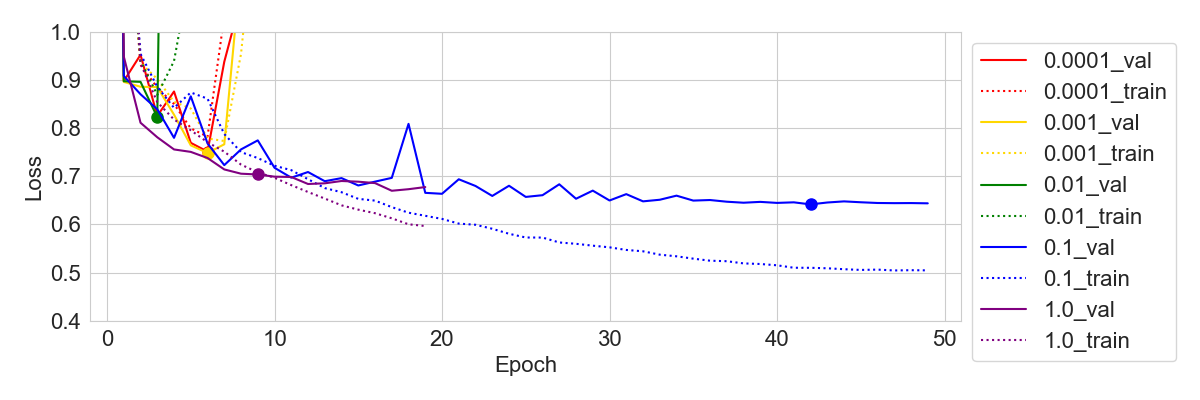
\includegraphics[height=55mm]{./figure/sec4/learning_curves/7/mel_loss.png}
        \caption{メルスペクトログラムについてのMAE Loss}
        \label{sec4:fig:learning_curve_method_7_val_mel_loss}
    \end{subfigure}
    \begin{subfigure}{\linewidth}
        \centering
        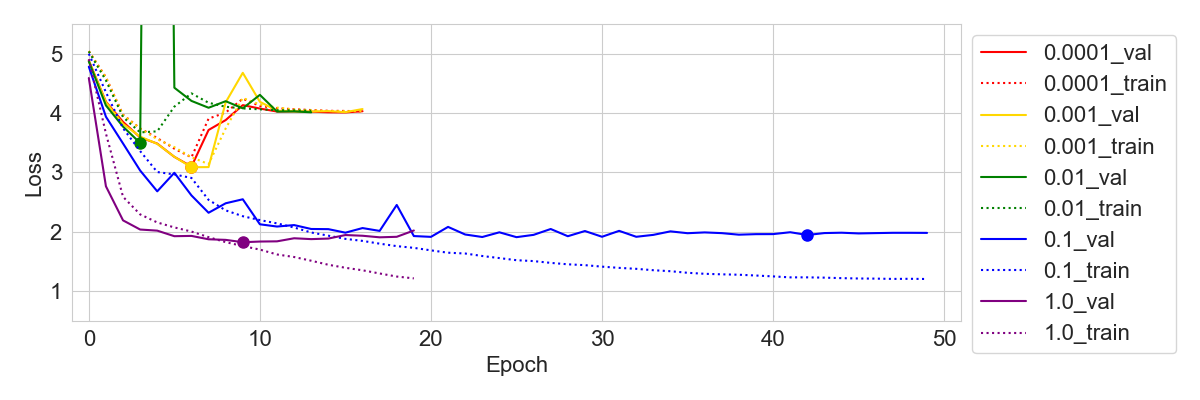
\includegraphics[height=55mm]{./figure/sec4/learning_curves/7/ssl_feature_cluster_loss.png}
        \caption{HuBERT離散特徴量についてのCross Entropy Loss}
        \label{sec4:fig:learning_curve_method_7_val_ssl_feature_cluster_loss}
    \end{subfigure}
    \begin{subfigure}{\linewidth}
        \centering
        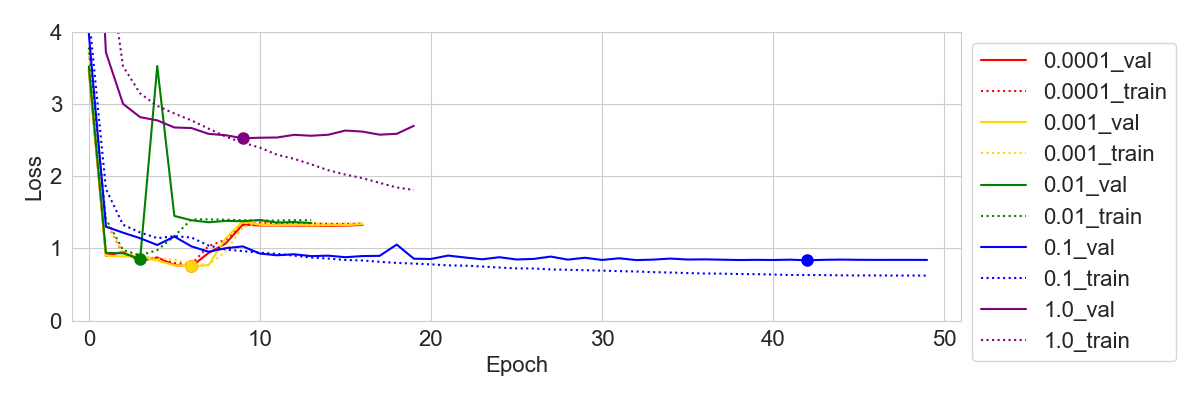
\includegraphics[height=55mm]{./figure/sec4/learning_curves/7/total_loss.png}
        \caption{損失の合計値}
        \label{sec4:fig:learning_curve_method_7_val_total_loss}
    \end{subfigure}
    \caption{ネットワークE2E(Randomized)における学習曲線}
    \label{sec4:fig:learning_curve_method_7_val_losses}
\end{figure}

\begin{table}[bt]
    \centering
    \caption{ネットワークB(Randomized・A-SingleTask)かつ,$\lossWeightHubDisc = 0.1$の場合における学習済み重みでネットワークAとネットワークBを初期化し,一度に学習させた場合の比較}
    \label{sec4:tab:obj_weights_e2e_pretrained}
    \begin{center}
        \renewcommand{\arraystretch}{1.0} % 行の高さ調整
        \setlength{\tabcolsep}{8pt}      % 列の幅調整
        \scalebox{1.0}{
            \begin{tabular}{|c|l|rr|}
                \hline
                \multicolumn{1}{|c|}{手法}         & \multicolumn{1}{c|}{$\learningRate_{\text{max}}$} & \multicolumn{1}{c}{WER [\%]} & \multicolumn{1}{c|}{話者類似度} \\
                \hline
                ネットワークE2E(Pretrained)            & $5.0 \times 10^{-4}$                              & 44.6                         & 0.851                      \\
                \textbf{ネットワークE2E(Pretrained)}   & $\mathbf{5.0 \times 10^{-5}}$                     & \textbf{43.5}                & \underline{\textbf{0.853}} \\
                ネットワークE2E(Pretrained)            & $5.0 \times 10^{-6}$                              & 43.6                         & \underline{0.853}          \\
                \hline
                ネットワークB(Randomized・A-SingleTask) & $5.0 \times 10^{-4}$                              & \underline{42.5}             & 0.847                      \\
                \hline
            \end{tabular}
        }
    \end{center}
\end{table}

\begin{figure}[bt]
    \centering
    \begin{subfigure}{\linewidth}
        \centering
        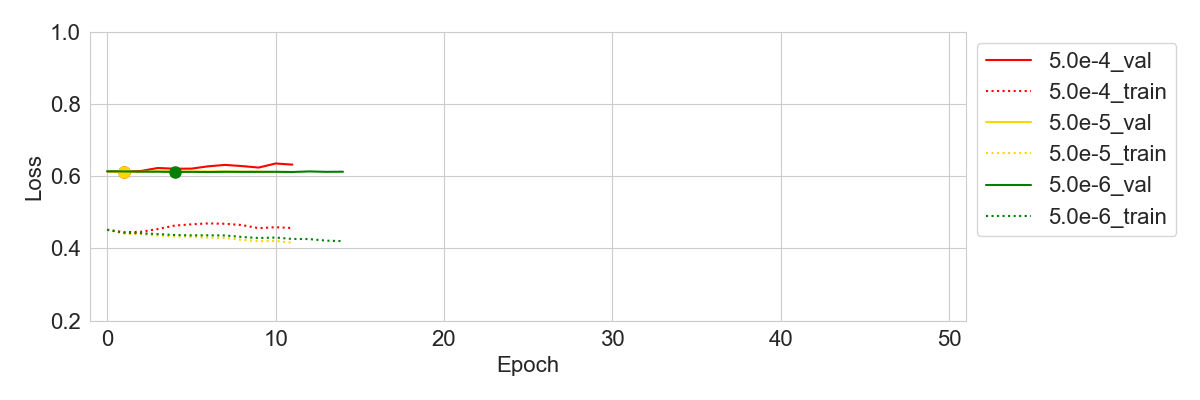
\includegraphics[height=55mm]{./figure/sec4/learning_curves/10_11_12/mel_loss.png}
        \caption{メルスペクトログラムについてのMAE Loss}
        \label{sec4:fig:learning_curve_method_10_11_12_val_mel_loss}
    \end{subfigure}
    \begin{subfigure}{\linewidth}
        \centering
        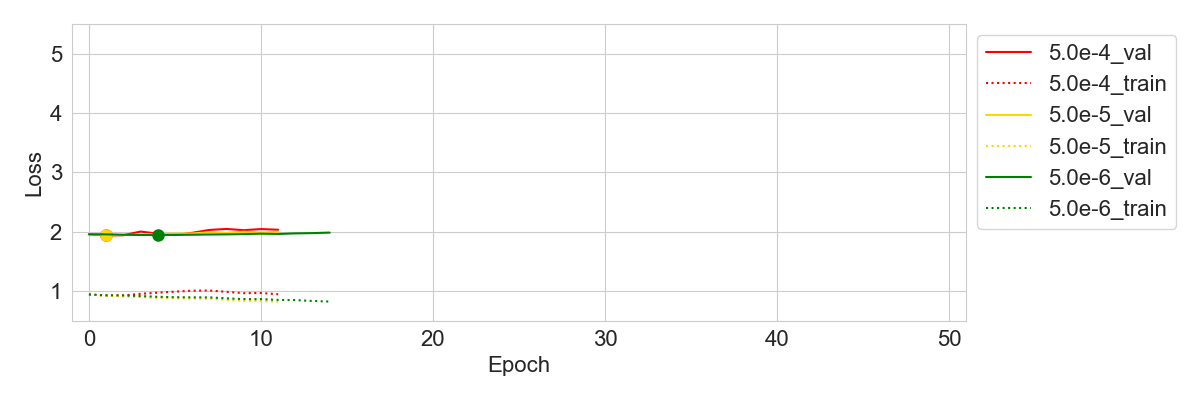
\includegraphics[height=55mm]{./figure/sec4/learning_curves/10_11_12/ssl_feature_cluster_loss.png}
        \caption{HuBERT離散特徴量についてのCross Entropy Loss}
        \label{sec4:fig:learning_curve_method_10_11_12_val_ssl_feature_cluster_loss}
    \end{subfigure}
    \begin{subfigure}{\linewidth}
        \centering
        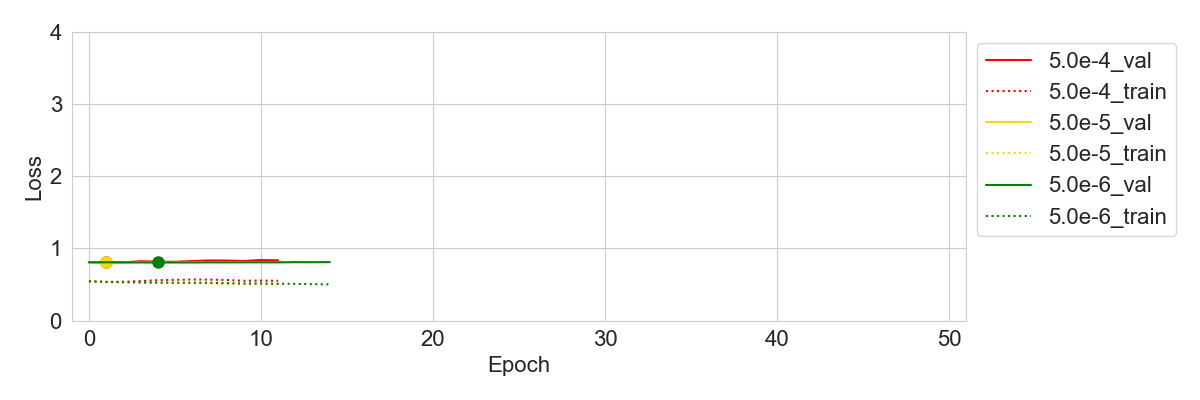
\includegraphics[height=55mm]{./figure/sec4/learning_curves/10_11_12/total_loss.png}
        \caption{損失の合計値}
        \label{sec4:fig:learning_curve_method_10_11_12_val_total_loss}
    \end{subfigure}
    \caption{ネットワークE2E(Pretrained)における学習曲線}
    \label{sec4:fig:learning_curve_method_10_11_12_val_losses}
\end{figure}

\clearpage

\subsubsection{主観評価}
主観評価実験では,\ref{sec4:sec:obj_1}節および\ref{sec4:sec:obj_2}節の検討結果を踏まえ,以下の五種類の音声を評価対象とした.
\begin{enumerate}
    \item ベースライン
    \item ネットワークB(Randomized)
    \item ネットワークB(Randomized・A-SingleTask)
    \item 分析合成
    \item 原音声
\end{enumerate}
ここで,ネットワークB(Randomized)およびネットワークB(Randomized・A-SingleTask)が,今回の実験を通して選択した提案手法の代表である.\ref{sec4:sec:sbj_explanation}節で述べたように,主観評価では音声の明瞭性と類似性の五段階評価を実施した.ダミー音声に対する評価値を誤った被験者は存在しなかったため,75人分のデータを統計処理に用いた.

まず,被験者に対するアンケートで得られた統計について,被験者の年齢層は21歳から62歳に渡った.年齢層の箱ひげ図を図\ref{sec4:fig:age}に示す.被験者の性別は男性32名,女性43名であった.また,実験に利用した音響機器はヘッドホンが19名,イヤホンが56名であった.
\begin{figure}[b]
    \centering
    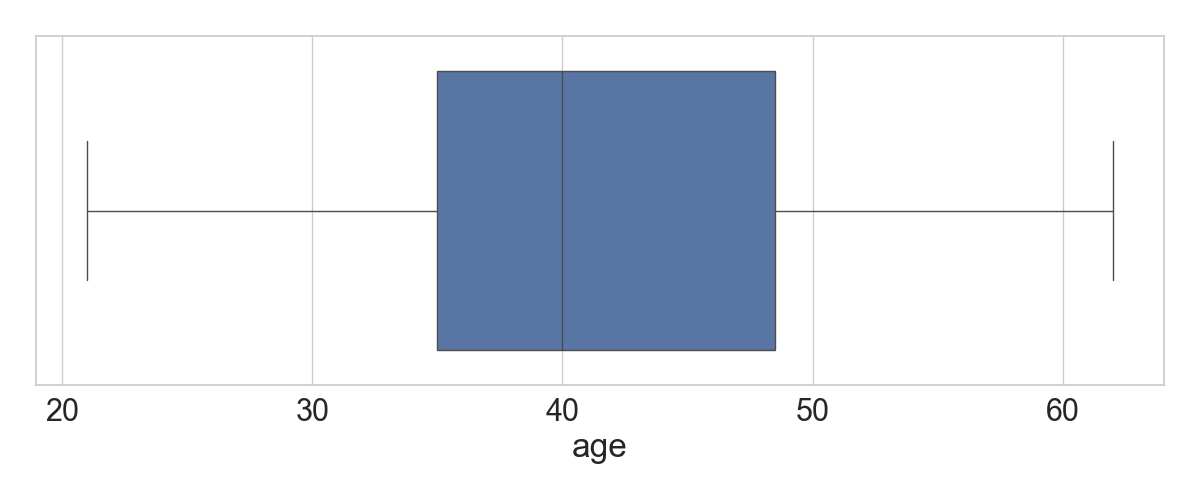
\includegraphics[height=50mm]{./figure/sec4/sbj/age.png}
    \caption{主観評価実験における被験者の年齢層}
    \label{sec4:fig:age}
\end{figure}

明瞭性と類似性の評価値について,手法ごとに平均値と95\%信頼区間を計算した結果を表\ref{sec4:tab:sbj_mean_ci}に示す.また,各手法の組み合わせについて,平均値の差の検定(Welchのt検定)を行った結果を表\ref{sec4:tab:sbj_int_p}, \ref{sec4:tab:sbj_sim_p}に示す.表における$\lr{i, j}$成分は,$i$行目の手法に対する評価値の母平均を$\mu_{i}$,$j$列目の手法に対する評価値の母平均を$\mu_{j}$とするとき,帰無仮説を$\mu_{i} = \mu_{j}$,対立仮説を$\mu_{i} > \mu_{j}$とした片側検定で計算されたp値に対し,Benjamini/Hochberg法による多重比較のための補正を行った結果である.ここで,表の文字列はそれぞれの以下の略称とする.
\begin{enumerate}
    \item GT: 原音声(Ground Truth)
    \item AbS: 分析合成(Analysis by Synthesis)
    \item B(Rand, A-S): ネットワークB(Randomized・A-SingleTask)
    \item B(Rand): ネットワークB(Randomized)
    \item Baseline: ベースライン
\end{enumerate}
また,本実験における有意水準は5\%とする.

まず,表\ref{sec4:tab:sbj_int_p}より,提案したネットワークB(Randomized)およびネットワークB(Randomized・A-SingleTask)は,ベースラインに対して明瞭性の評価値が有意に高いことがわかる.これより,二つの提案手法はどちらもベースラインより明瞭性の高い合成音声を実現できたと考えられる.一方,提案手法二つの間には有意差がないことも分かる.これより,ネットワークAの学習方法の違いは明瞭性に有意差をもたらさなかったと言える.次に,表\ref{sec4:tab:sbj_sim_p}より,提案したネットワークB(Randomized)およびネットワークB(Randomized・A-SingleTask)は,ベースラインに対して類似性の評価値が有意に高いことがわかる.これより,二つの提案手法はどちらもベースラインより類似性の高い合成音声を実現できたと考えられる.また,ここでは提案手法二つの間にも有意差があることが分かる.これより,ネットワークAの学習方法の違いは類似性に有意な差をもたらしたと言える.以上のことから,ネットワークB(Randomized・A-SingleTask)が明瞭性・類似性の両面において,優れた合成音声を実現したと考えられる.

\begin{table}[bt]
    \centering
    \caption{主観評価実験の結果より計算した標本平均と95\%信頼区間}
    \label{sec4:tab:sbj_mean_ci}
    \begin{center}
        \renewcommand{\arraystretch}{1.0} % 行の高さ調整
        \setlength{\tabcolsep}{8pt}      % 列の幅調整
        \scalebox{0.95}{
            \begin{tabular}{|c|l|rr|}
                \hline
                \multicolumn{1}{|c|}{手法}         & \multicolumn{1}{c|}{$\lossWeightHubDisc$} & \multicolumn{1}{c}{明瞭性} & \multicolumn{1}{c|}{類似性} \\
                \hline
                ベースライン                           & 0.001                                     & $2.37 \pm 0.07$         & $2.92 \pm 0.08$          \\
                ネットワークB(Randomized)              & 0.1                                       & $2.76 \pm 0.07$         & $3.04 \pm 0.08$          \\
                ネットワークB(Randomized・A-SingleTask) & 0.1                                       & $2.82 \pm 0.08$         & $3.18 \pm 0.08$          \\
                \hline
                分析合成                             & \multicolumn{1}{c|}{-}                    & $4.75 \pm 0.04$         & $4.31 \pm 0.07$          \\
                原音声                              & \multicolumn{1}{c|}{-}                    & $4.87 \pm 0.03$         & $4.71 \pm 0.05$          \\
                \hline
            \end{tabular}
        }
    \end{center}
\end{table}

\begin{table}[bt]
    \centering
    \caption{主観評価実験の結果より計算した平均値の差の検定におけるp値(明瞭性)}
    \label{sec4:tab:sbj_int_p}
    \begin{center}
        \renewcommand{\arraystretch}{1.0} % 行の高さ調整
        \setlength{\tabcolsep}{8pt}      % 列の幅調整
        \scalebox{0.95}{
            \begin{tabular}{|c|rrrr|}
                \hline
                \multicolumn{1}{|c|}{} & \multicolumn{1}{c}{AbS} & \multicolumn{1}{c}{B(Rand, A-S)} & \multicolumn{1}{c}{B(Rand)} & \multicolumn{1}{c|}{Baseline} \\
                \hline
                GT                     & $6.67 \times 10^{-6}$   & $6.17 \times 10^{-262}$          & $2.84 \times 10^{-289}$     & $0$                           \\
                AbS                    & \multicolumn{1}{c}{-}   & $3.22 \times 10^{-243}$          & $2.40 \times 10^{-270}$     & $0$                           \\
                B(Rand, A-S)           & \multicolumn{1}{c}{-}   & \multicolumn{1}{c}{-}            & $1.23 \times 10^{-1}$       & $7.07 \times 10^{-17}$        \\
                B(Rand)                & \multicolumn{1}{c}{-}   & \multicolumn{1}{c}{-}            & \multicolumn{1}{c}{-}       & $1.12 \times 10^{-13}$        \\
                \hline
            \end{tabular}
        }
    \end{center}
\end{table}

\begin{table}[bt]
    \centering
    \caption{主観評価実験の結果より計算した平均値の差の検定におけるp値(類似性)}
    \label{sec4:tab:sbj_sim_p}
    \begin{center}
        \renewcommand{\arraystretch}{1.0} % 行の高さ調整
        \setlength{\tabcolsep}{8pt}      % 列の幅調整
        \scalebox{0.95}{
            \begin{tabular}{|c|rrrr|}
                \hline
                \multicolumn{1}{|c|}{} & \multicolumn{1}{c}{AbS} & \multicolumn{1}{c}{B(Rand, A-S)} & \multicolumn{1}{c}{B(Rand)} & \multicolumn{1}{c|}{Baseline} \\
                \hline
                GT                     & $1.24 \times 10^{-18}$  & $5.86 \times 10^{-160}$          & $9.90 \times 10^{-174}$     & $1.28 \times 10^{-205}$       \\
                AbS                    & \multicolumn{1}{c}{-}   & $3.11 \times 10^{-83}$           & $1.73 \times 10^{-97}$      & $3.58 \times 10^{-120}$       \\
                B(Rand, A-S)           & \multicolumn{1}{c}{-}   & \multicolumn{1}{c}{-}            & $1.13 \times 10^{-2}$       & $5.46 \times 10^{-6}$         \\
                B(Rand)                & \multicolumn{1}{c}{-}   & \multicolumn{1}{c}{-}            & \multicolumn{1}{c}{-}       & $2.13 \times 10^{-2}$         \\
                \hline
            \end{tabular}
        }
    \end{center}
\end{table}